\documentclass[tikz,border=4pt]{standalone}
\usepackage{pgfplots}
\pgfplotsset{compat=1.18}

\begin{document}
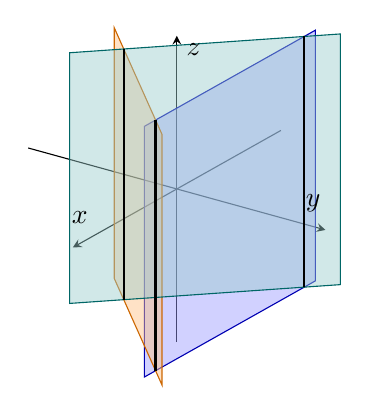
\begin{tikzpicture}
\begin{axis}[
    view={125}{25},
    axis lines=center,
    xlabel={$x$},
    ylabel={$y$},
    zlabel={$z$},
    xmin=-2.8, xmax=2.8,
    ymin=-2.8, ymax=2.8,
    zmin=-2.2, zmax=2.2,
    xtick=\empty, ytick=\empty, ztick=\empty,
    width=8cm, height=8cm,
    clip=false
]

% Plane 1: y = 1 (blue)
\addplot3[
    surf,
    shader=flat,
    draw=blue!70!black,
    fill=blue!40,
    fill opacity=0.45,
    samples=2,
    domain=-2.3:2.3,
    y domain=-1.8:1.8
] ({x}, {1}, {y});

% Plane 2: y = x - 1 (orange)
\addplot3[
    surf,
    shader=flat,
    draw=orange!80!black,
    fill=orange!50,
    fill opacity=0.45,
    samples=2,
    domain=-0.6:2.4,
    y domain=-1.8:1.8
] ({x}, {x - 1}, {y});

% Plane 3: y = -x - 1 (teal)
\addplot3[
    surf,
    shader=flat,
    draw=teal!80!black,
    fill=teal!40,
    fill opacity=0.45,
    samples=2,
    domain=-2.4:0.6,
    y domain=-1.8:1.8
] ({x}, {-x - 1}, {y});

% Three parallel vertical pairwise intersection lines
\addplot3[domain=-1.8:1.8, samples=2, thick, black] ({2}, {1}, {x});
\addplot3[domain=-1.8:1.8, samples=2, thick, black] ({-2}, {1}, {x});
\addplot3[domain=-1.8:1.8, samples=2, thick, black] ({0}, {-1}, {x});

\end{axis}
\end{tikzpicture}
\end{document}
